\documentclass[compress, aspectratio=32]{beamer}
\usepackage[utf8]{inputenc}
\usepackage{graphicx} % Required for inserting images
\graphicspath{ {./images/} }
\usepackage{amsmath}
\usepackage{mathspec}
\usepackage{xeCJK}
\usepackage{multicol}
\usepackage{float}
\usepackage{soul}
\usepackage{hyperref}
\usepackage{caption}
\usepackage{subcaption}
\usepackage{ulem}
\usepackage{listings}
\usepackage[backend=biber, citestyle=authoryear, sorting=none]{biblatex}
\addbibresource{ref.bib}

\useinnertheme{circles}
\useoutertheme[subsection=true, footline=authortitle]{miniframes}
%\usecolortheme{seagull}
\usefonttheme{structurebold}

\setmainfont{Sabon LT Pro}
\setsansfont{SF Pro Display}
%\setmathfont(Digits,Latin){Goldman Sans}
\setmonofont{IBM Plex Mono}

\AtBeginSection[]
{
    
  \begin{frame}[allowframebreaks]
    
    \tableofcontents[currentsection]
    
  \end{frame}
}

% \AtBeginSubsection[]{
%     \begin{frame}[allowframebreaks]
%         \tableofcontents[currentsubsection]
%     \end{frame}
% }

\title[IoT Intro]{Intro to Internet of Things}
\subtitle{with ESP/Arduino}
\author{Ben Cheng}
\institute{RISD ID}
\date{\today}

\setbeamertemplate{navigation symbols}{\insertframenumber/\inserttotalframenumber}
\setbeamertemplate{title page}{
    \vbox{}
    \vfill
    \begin{beamercolorbox}[sep=8pt,left]{title}
        \begin{columns}
            \begin{column}[]{0.7\textwidth}
                \usebeamerfont{title}\inserttitle\par
        \ifx\insertsubtitle\@empty
        \else
          \vskip0.25em
          {\usebeamerfont{subtitle}\usebeamercolor[fg]{subtitle}\insertsubtitle\par}%
        \fi   
            \end{column}
            \begin{column}[]{0.1\textwidth}
                
\includegraphics[width=\textwidth]{IDSB-logo.png}
            \end{column}
        \end{columns}
          
      \end{beamercolorbox}
    \vskip1em\par
    \begin{beamercolorbox}[sep=8pt,left]{author}
      \usebeamerfont{author}\insertauthor
    \end{beamercolorbox}
    \begin{beamercolorbox}[sep=8pt,left]{institute}
        \usebeamerfont{institute}\insertinstitute
    \end{beamercolorbox}
    \begin{beamercolorbox}[sep=8pt,right]{date}
        \usebeamerfont{date}\insertdate
    \end{beamercolorbox}\vskip0.5em
    {\usebeamercolor[fg]{titlegraphic}\inserttitlegraphic\par}
    \vfill
}

\definecolor{customColor}{RGB}{90, 158, 108}
\setbeamercolor*{palette primary}{fg=customColor!60!black,bg=white!85!customColor}
\setbeamercolor*{palette secondary}{fg=customColor!70!black,bg=white!60!customColor}
\setbeamercolor*{palette tertiary}{bg=customColor!80!black,fg=white!50!customColor}
\setbeamercolor*{palette quaternary}{fg=customColor,bg=white!20!customColor}

\setbeamercolor*{sidebar}{fg=customColor,bg=customColor!75!white}

\setbeamercolor*{palette sidebar primary}{fg=customColor!10!black}
\setbeamercolor*{palette sidebar secondary}{fg=white}
\setbeamercolor*{palette sidebar tertiary}{fg=customColor!50!black}
\setbeamercolor*{palette sidebar quaternary}{fg=white!10!customColor}

\setbeamercolor*{titlelike}{parent=palette primary}
\setbeamercolor{frametitle}{bg=white!90!customColor}
\setbeamercolor{frametitle right}{bg=white!60!customColor}

\setbeamercolor{block title}{parent=palette tertiary}
\setbeamercolor{block body}{bg=white!90!customColor}

\setbeamercolor*{item projected}{parent=palette primary}%fg=black,bg=black!20}

\setbeamercolor*{normal text}{fg=black,bg=white}
\setbeamercolor*{alerted text}{fg=black}
\setbeamercolor*{example text}{fg=black}
\setbeamercolor*{structure}{fg=black}

\setbeamercolor{author in head/foot}{parent=title in head/foot}

\lstdefinestyle{mystyle}{basicstyle=\ttfamily\scriptsize, numbers=left, frame=lines, breaklines=true, showstringspaces=false}
\lstset{style=mystyle}

\begin{document}

\frame{\titlepage}

\begin{frame}[allowframebreaks]{Outline}
    \tableofcontents
\end{frame}

\section{Internet}
\begin{frame}{What is the internet?}
    A network connecting an enormous number of computing devices.
    \par How to operate a network like this?
    \begin{itemize}
        \item Wire them all toghether?
        \item Who connect to whom?
        \item How many steps to send a message?
    \end{itemize}
\end{frame}

\begin{frame}
    \frametitle{Hierachy+Protocol}
    \begin{itemize}
        \item Devices are connected by hierachy.
        \item Different devices are connected via different protocols.
        \item Data is coded according to the layers of the internet model.
    \end{itemize}
    \begin{figure}
        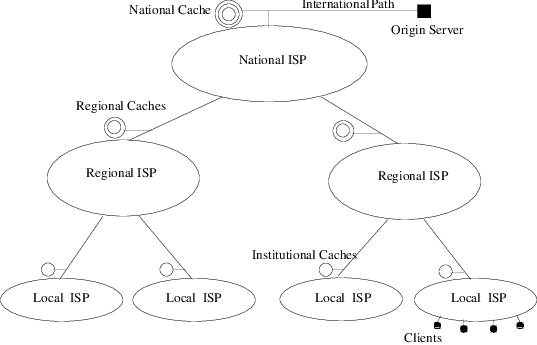
\includegraphics[width=0.5\textwidth]{Internet-topology-hierarchical-structure.png}
        \caption*{(\cite{inproceedings})}
    \end{figure}
\end{frame}

\begin{frame}
    \frametitle{Layers of the internet}
    \begin{columns}
        \begin{column}[]{0.3\linewidth}
            \begin{enumerate}
                \item HTTP request
                \item TCP port
                \item IP address
                \item MAC address
                \item Wireless LAN
            \end{enumerate}
        \end{column}
        \begin{column}[]{0.7\linewidth}
            \begin{figure}
                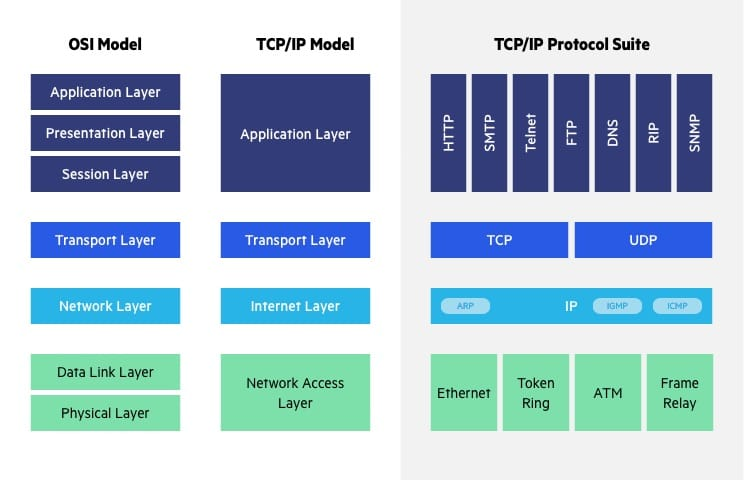
\includegraphics[width=0.9\textwidth]{OSI-vs.-TCPIP-models.jpg}
                \caption*{(Imperva)}
            \end{figure}
        \end{column}
    \end{columns}
\end{frame}

\begin{frame}
    \frametitle{(Almost) Everything is a HTTP request}
    \begin{columns}
        \begin{column}[]{0.3\textwidth}
            HTTP follows a client-server model.
            \begin{itemize}
                \item Client request
                \item Serve respond
            \end{itemize}
        \end{column}
        \begin{column}[]{0.7\textwidth}
            \begin{figure}
                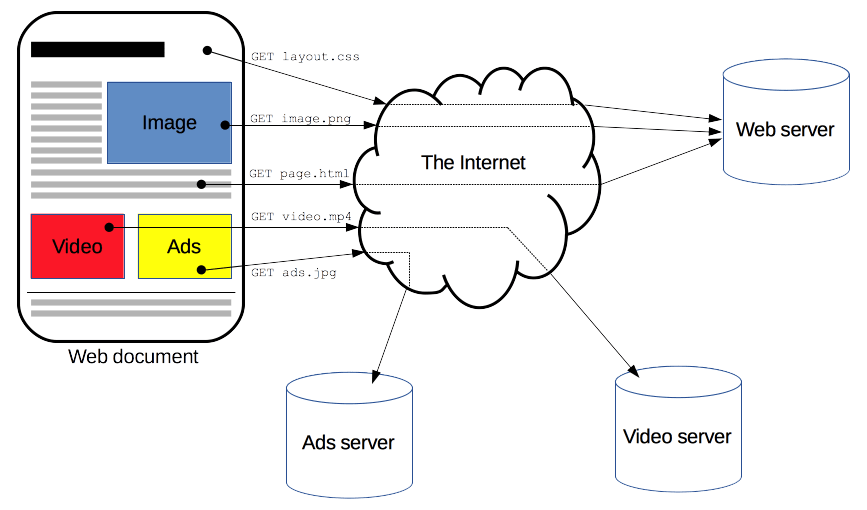
\includegraphics[width=\textwidth]{fetching_a_page.png}
                \caption*{(Mozilla)}
            \end{figure}            
        \end{column}
    \end{columns}
\end{frame}

\begin{frame}
    \frametitle{HTTP request}
    \begin{columns}
        \begin{column}[]{0.5\textwidth}
            \begin{itemize}
                \item Method: GET, POST
                \item Path
                \item Header
                \item Body
            \end{itemize}
        \end{column}
        \begin{column}[]{0.5\textwidth}
            \begin{figure}
                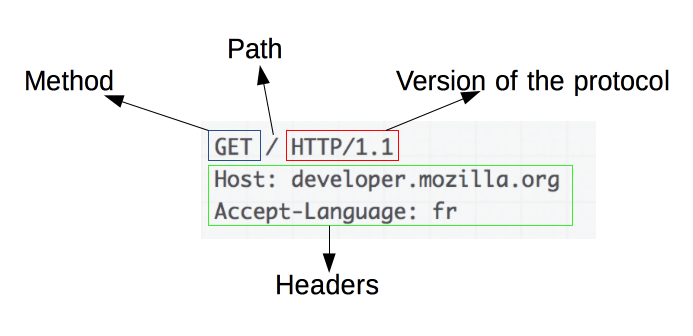
\includegraphics[width=\textwidth]{http_request.png}
                \caption*{(Mozilla)}
            \end{figure}
        \end{column}
    \end{columns}
\end{frame}

\section[IoT]{Internet of Things}

\begin{frame}
    \frametitle{Components}
    \begin{columns}
        \begin{column}[]{0.4\textwidth}
            \begin{enumerate}
                \item Node
                \item Gateway
                \item Cloud
                \item Database
            \end{enumerate}            
        \end{column}
        \begin{column}{0.6\textwidth}
            \begin{figure}
                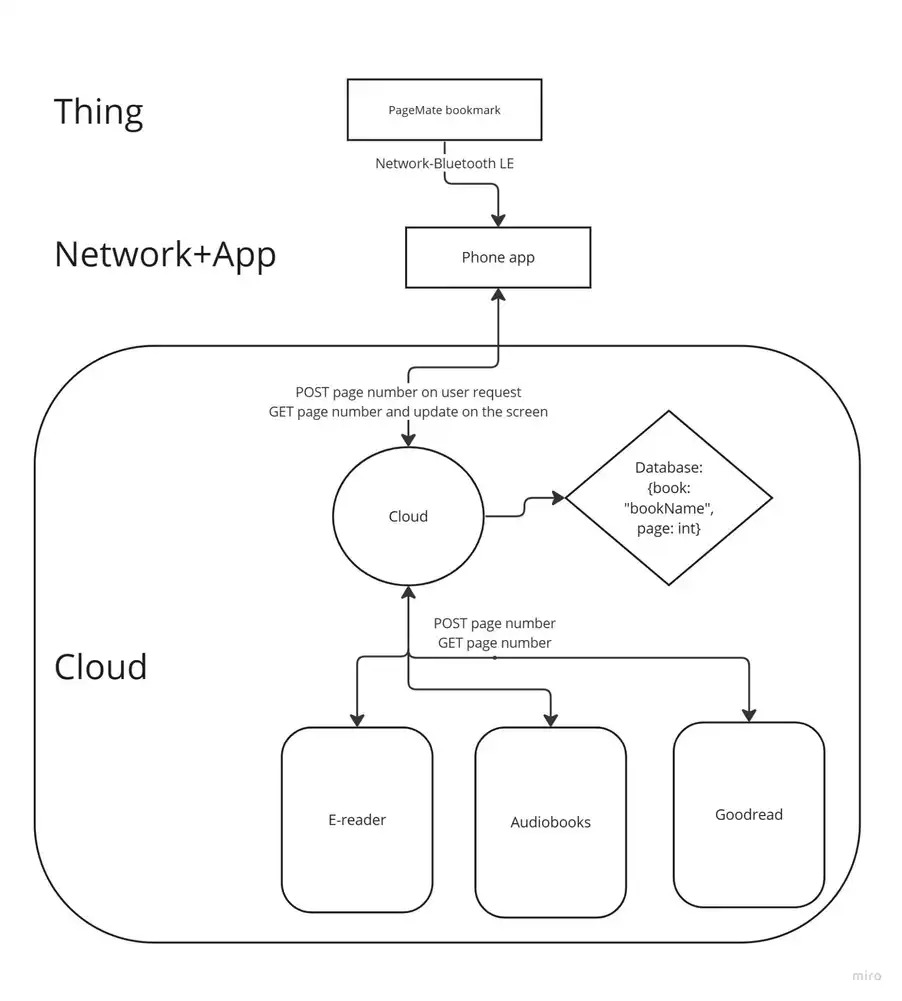
\includegraphics[height=0.8\textheight]{architecture.jpg}
            \end{figure}
        \end{column}
    \end{columns}
\end{frame}

\begin{frame}
    \frametitle{Example: Power Cable Monitoring}
    \begin{columns}
        \begin{column}{0.4\textwidth}
            \begin{itemize}
                \item Long distance between towers
                \item Connection hard/dangerous to install
            \end{itemize}
        \end{column}
        \begin{column}{0.6\textwidth}
            \begin{figure}
                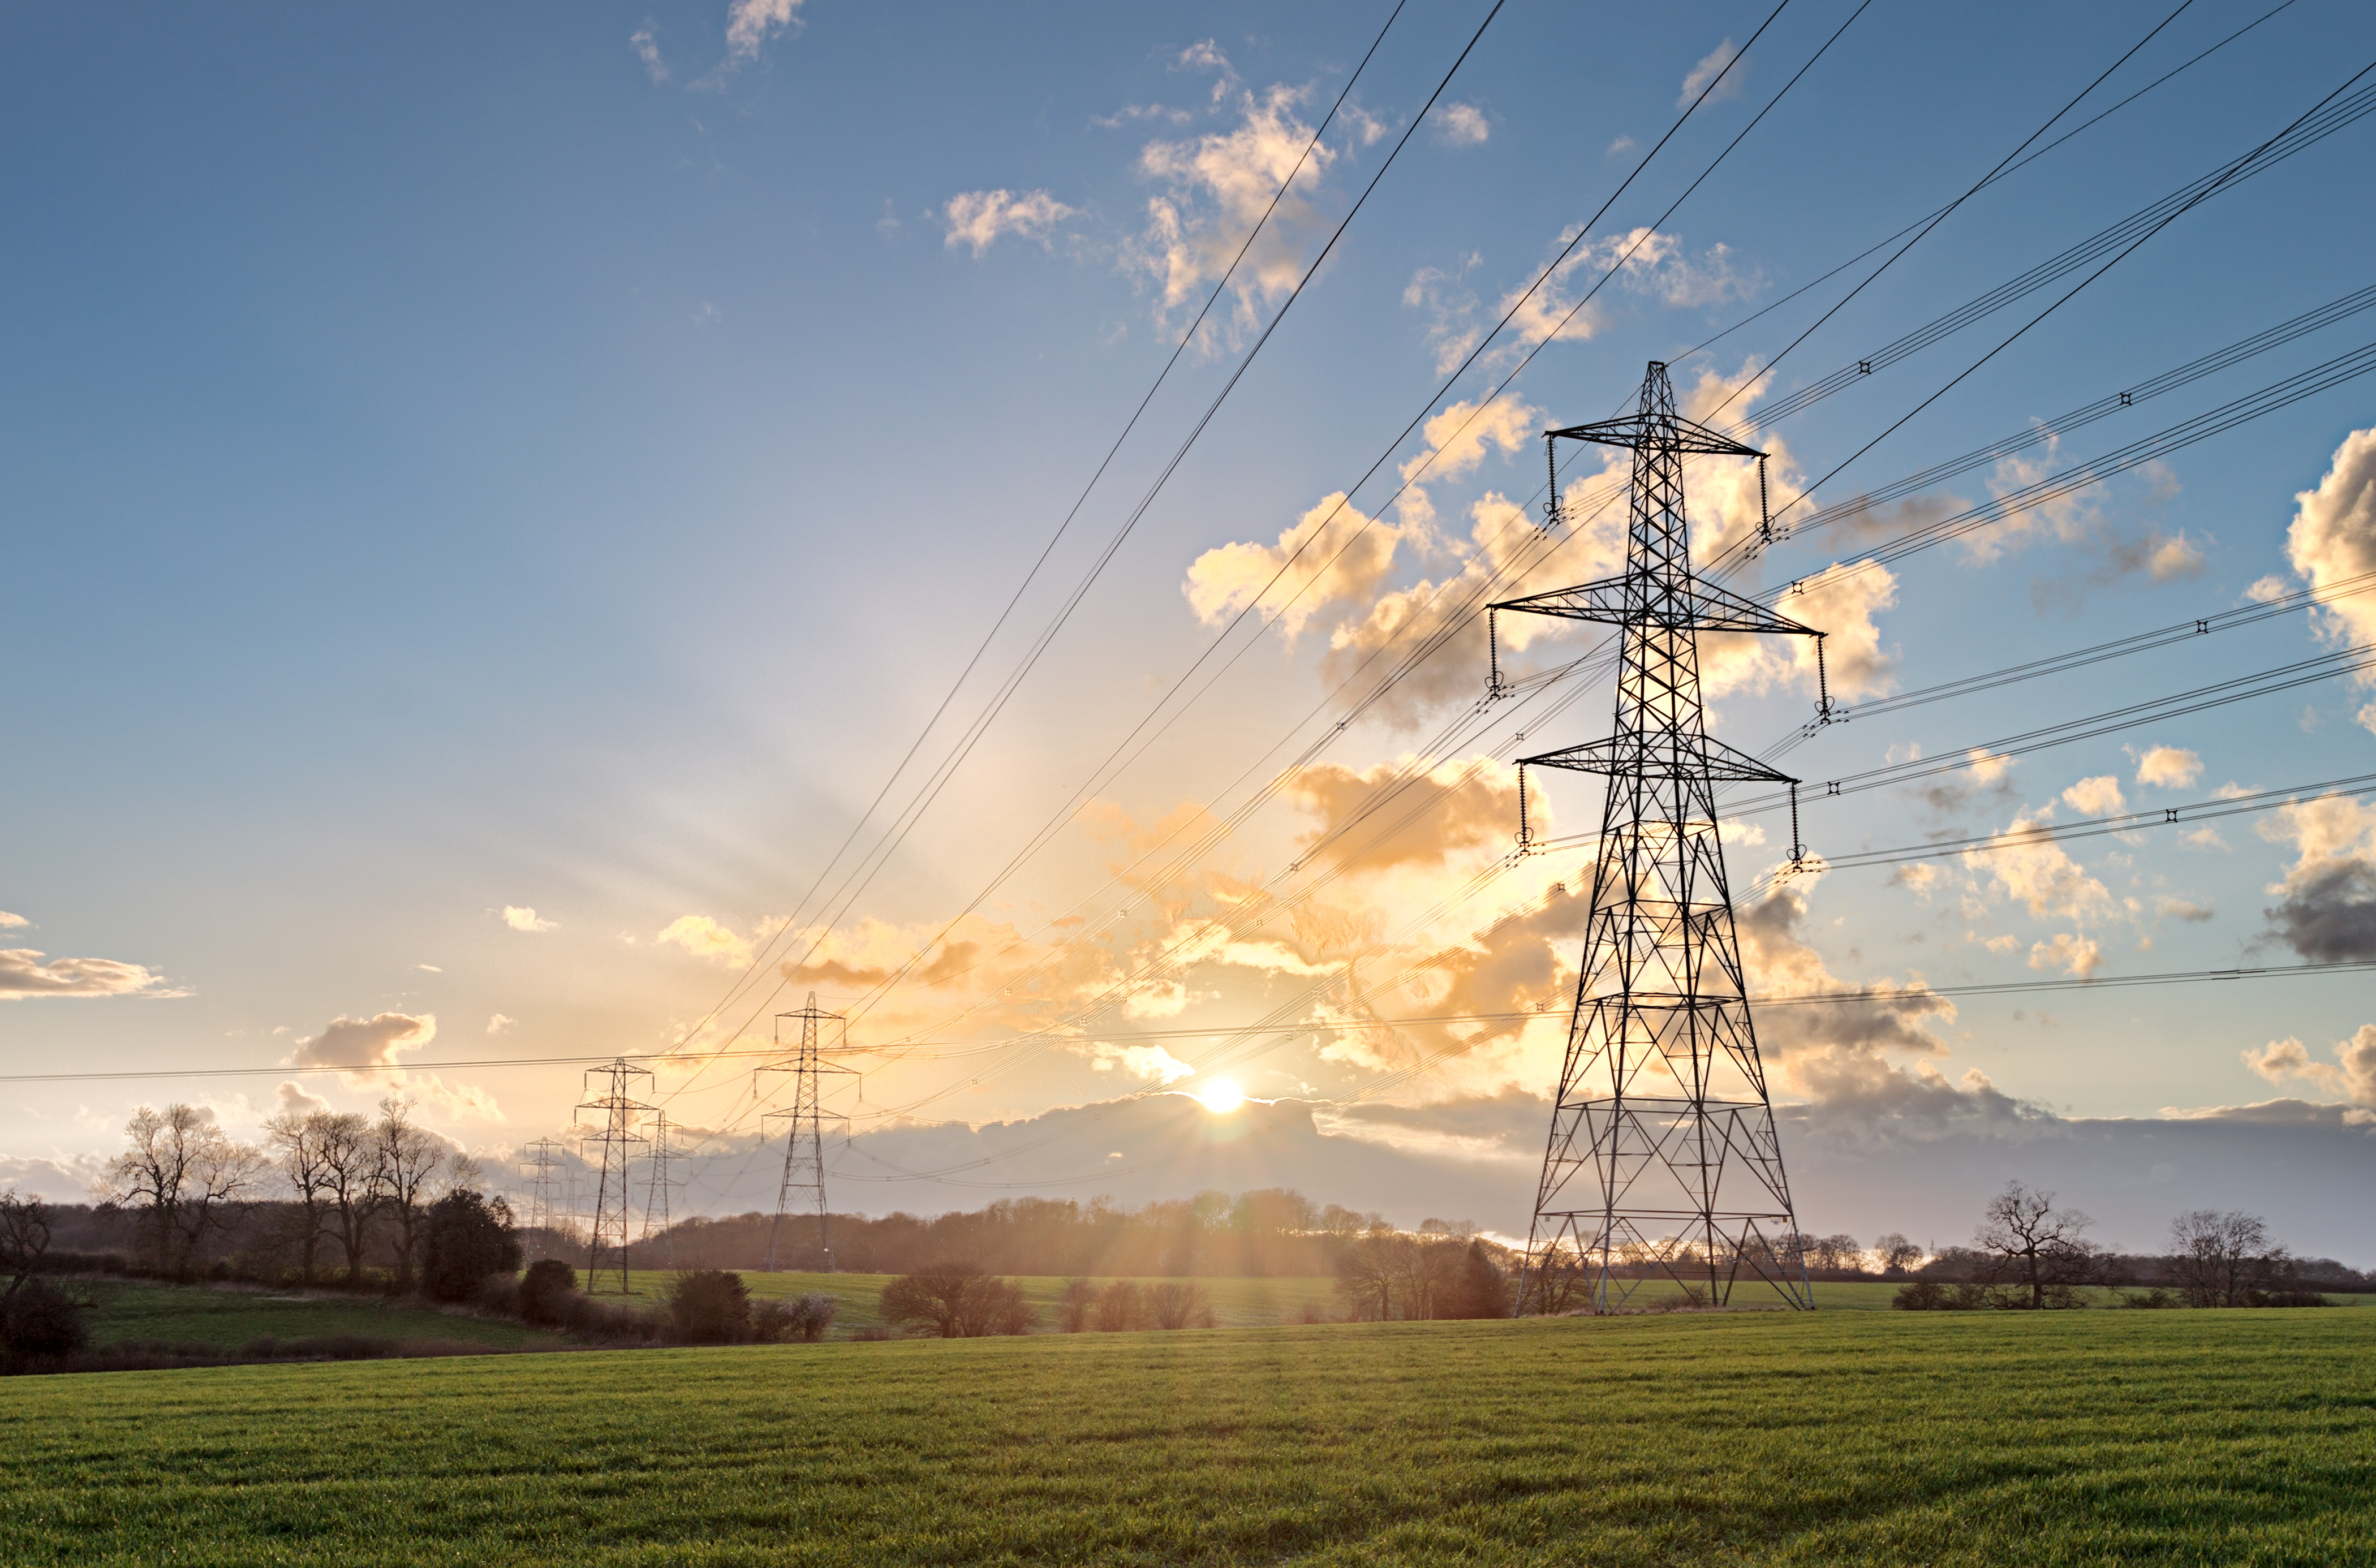
\includegraphics[width=\textwidth]{AdobeStock_133386757.jpeg}
            \end{figure}
        \end{column}
    \end{columns}
\end{frame}

\begin{frame}
    \frametitle{What's covered today?}
    \begin{itemize}
        \item Node
        \item \st{Gateway}: your phone
        \item \st{Cloud}: a basic Express app
        \item \st{Database}: MangoDB, mySQL
    \end{itemize}
\end{frame}

\section{Node: ESP}

\begin{frame}
    \frametitle{What is a computer?}
    \begin{columns}
        \begin{column}{0.4\textwidth}
            \begin{enumerate}
                \item Processing Unit: ALU
                    \begin{itemize}
                        \item Arithmetic operation
                        \item Signal processing
                        \item Conditional decision
                    \end{itemize}
                \item Memory: hierachy
                \item I/O
                \begin{itemize}
                    \item ADC
                    \item USB
                    \item Wireless
                \end{itemize}
            \end{enumerate}
            ESP32 is a system on chip (SoC).
        \end{column}
        \begin{column}{0.6\textwidth}
            \begin{figure}
                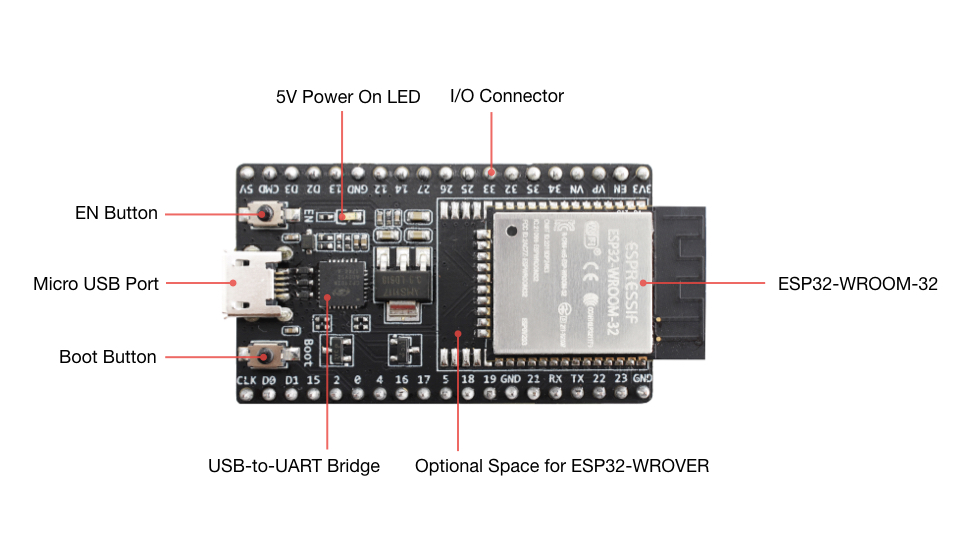
\includegraphics[width=0.9\textwidth]{esp32-devkitc-functional-overview.jpg}
                \caption*{(Espressif)}
            \end{figure}
        \end{column}
    \end{columns}
\end{frame}

\begin{frame}
    \frametitle{Embedded Computer}
    \begin{columns}
        \begin{column}[]{0.4\textwidth}
            \begin{itemize}
                \item Does not have operating system.
                \item Application is embedded into the firmware.
            \end{itemize}
        \end{column}
        \begin{column}[]{0.6\textwidth}
            \begin{figure}
                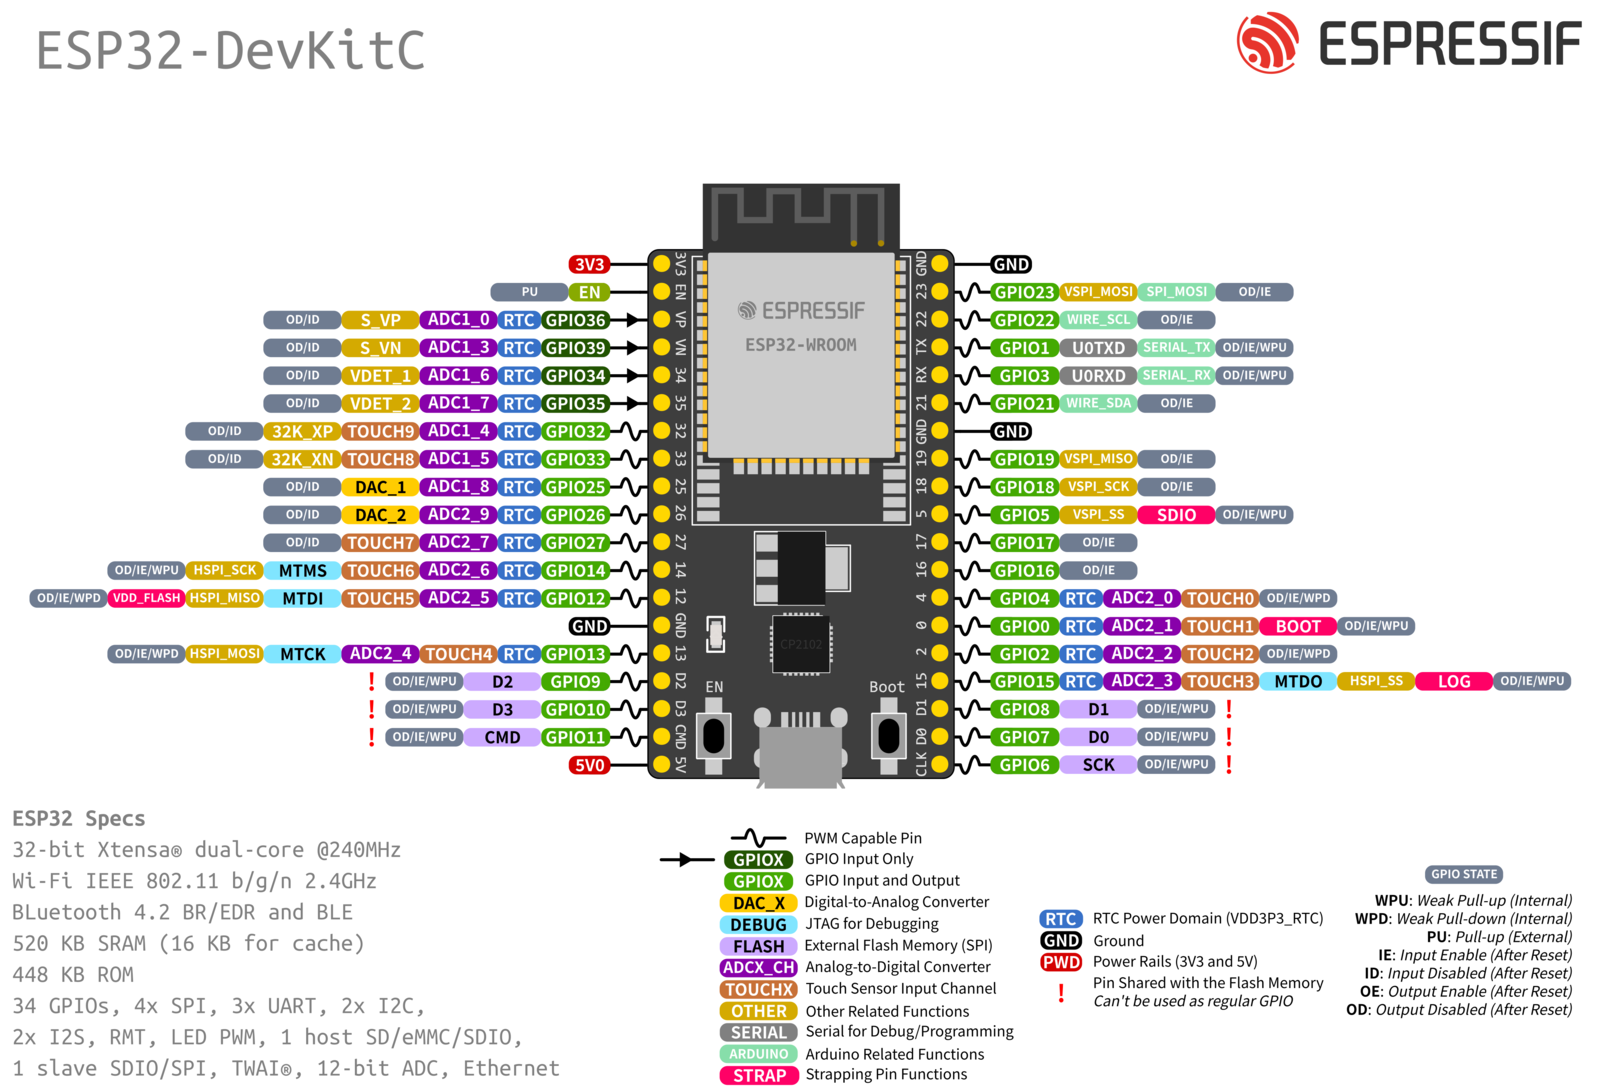
\includegraphics[width=\textwidth]{esp32-devkitC-v4-pinout.png}
                \caption*{(Espressif)}
            \end{figure}
        \end{column}
    \end{columns}
\end{frame}

\section{Implementation}

\subsection{ESP8266}
\begin{frame}
    \frametitle{ESP8266}
    \begin{figure}
        \centering
        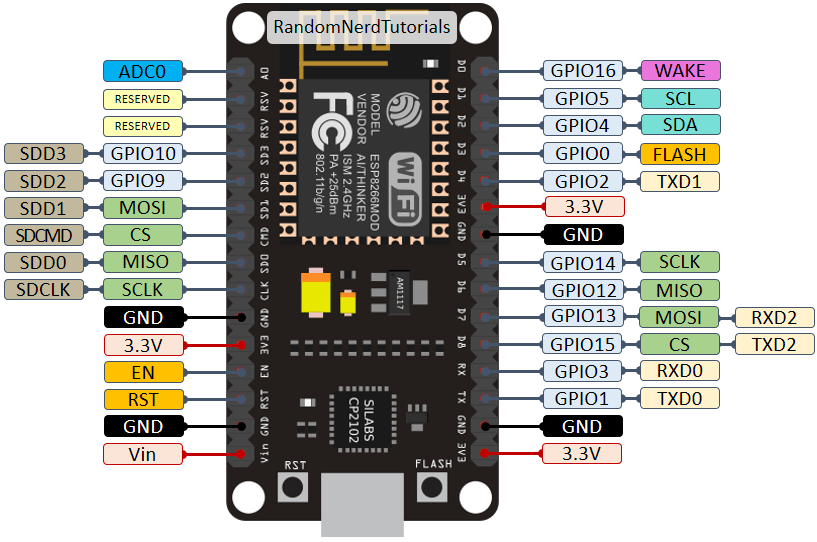
\includegraphics[height=0.7\textheight]{ESP8266-NodeMCU-kit-12-E-pinout-gpio-pin.png}
        \caption*{(Random Nerd Tutorials)}
    \end{figure}
\end{frame}
\begin{frame}[fragile]
    \frametitle{Checking and Basic Code Structure}
    \begin{enumerate}
        \item Connect ESP8266 to your computer and open Arduino IDE
        \item Select board NodeMCU 1.0 (ESP12E) and choose the right port in Tools
        \item Open File>Example>ESP8266>Blink and uplaod
    \end{enumerate}
    \begin{lstlisting}[language=c]
void setup() {
  pinMode(LED_BUILTIN, OUTPUT);  
}

// the loop function runs over and over again forever
void loop() {
  digitalWrite(LED_BUILTIN, LOW);  
  delay(1000);                      
  digitalWrite(LED_BUILTIN, HIGH);  
  delay(2000);   
}                   
    \end{lstlisting}
    
\end{frame}

\subsection{Servo}
\begin{frame}
    \frametitle{Servo Motor}
    \begin{columns}
        \begin{column}[]{0.5\textwidth}
            \begin{itemize}
                \item Small
                \item Powered by internal 3.3V
                \item Easy to control
                \item Only rotate 180 degree
            \end{itemize}
        \end{column}
        \begin{column}[]{0.5\textwidth}
            \begin{figure}
                \centering
                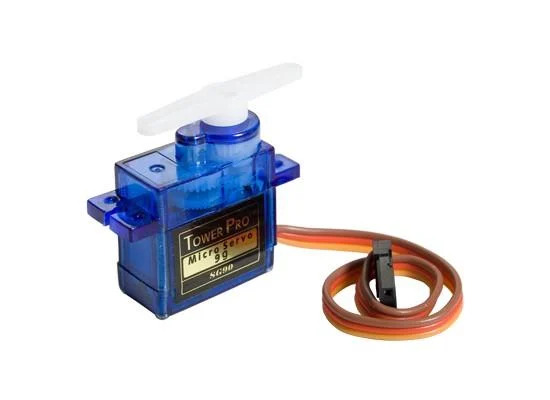
\includegraphics[width=\textwidth]{servo.jpg}
                \caption*{(ElectronicWings)}
            \end{figure}
        \end{column}
    \end{columns}
\end{frame}
\begin{frame}[fragile]
    \frametitle{Sweep}
    \begin{itemize}
        \item Orange to GPIO14=D4, red to 3V3, brown to GND
    \end{itemize}
    \begin{lstlisting}[language=c]
#include <Servo.h>
Servo myservo;
void setup() {
    myservo.attach(14);
}
void loop() {
    int pos = 0;
    for (pos = 0; pos <= 180; pos += 1) {  
        myservo.write(pos);  
        delay(30);           
    }
    for (pos = 180; pos >= 0; pos -= 1) {  
        myservo.write(pos);                  
        delay(30);
    }
}
    \end{lstlisting}
\end{frame}

\subsection{Ultrasonic Sensor}
\begin{frame}[fragile]
    \frametitle{Ultrasonic Sensor}
    \begin{itemize}
        \item Includes an emitter and a receiver.
        \item Calculate distance by time taken to travel from emitter to receiver.
        \item Ultrasonic is a mechanical wave
    \end{itemize}
    \begin{lstlisting}[language=c]
#include <Servo.h>
Servo myservo;
const int trigPin = 0; //connect trig pin to GPIO0=D3
const int echoPin = 4; //connect echo pin to GPIO4=D2

float duration, distance;
    \end{lstlisting}
\end{frame}

\begin{frame}[fragile]
    \frametitle{Setup and Serial Communication}
    \begin{itemize}
        \item Serial sends text to your computer
        \item Tools>Serial Monitor>Set correct baud rate
    \end{itemize}
    \begin{lstlisting}[language=c, firstnumber=last]
void setup() {
    myservo.attach(14);
    pinMode(trigPin, OUTPUT);
    pinMode(echoPin, INPUT);
    
    Serial.begin(115200);
    Serial.println("Hello World!");
}
    \end{lstlisting}
\end{frame}

\begin{frame}[fragile]
    \frametitle{Calculate distance and send via serial}
    \begin{lstlisting}[language=c, firstnumber=last]
void loop() {
    digitalWrite(trigPin, LOW);
    delayMicroseconds(2);
    digitalWrite(trigPin, HIGH);
    delayMicroseconds(10);
    digitalWrite(trigPin, LOW);

    duration = pulseIn(echoPin, HIGH);
    distance = (duration*.0343)/2;
    Serial.print("Distance: ");
    Serial.println(distance);
}
    \end{lstlisting}
\end{frame}

\subsection{DHT22}
\begin{frame}[fragile]
    \frametitle{DHT22}
    \begin{itemize}
        \item An integrated temperature and humidity sensor
        \item Easy to use with complete library
    \end{itemize}
    \begin{lstlisting}[language=c, firstnumber=1]
#include <Servo.h>
#include "DHT.h"

#define DHTPIN 4 //GPIO4=D2
#define DHTTYPE DHT22

Servo myservo;
DHT dht(DHTPIN, DHTTYPE);
    \end{lstlisting}
\end{frame}

\begin{frame}[fragile]
    \frametitle{Setup}
    \begin{lstlisting}[language=c, firstnumber=last]
void setup() {
    myservo.attach(14);
    dht.begin();
    
    Serial.begin(115200);
    Serial.println("Hello World!");
}
    \end{lstlisting}
\end{frame}

\begin{frame}[fragile]
    \frametitle{Loop}
    \begin{lstlisting}[language=c, firstnumber=last]
void loop() {
    float t = dht.readTemperature(true);
    if (isnan(t)) {
      Serial.println("DHT failed");
    }
    else {
      Serial.println("Temp: " + String(t));
    }
}
    \end{lstlisting}
\end{frame}

\subsection{HTTP}
\begin{frame}[fragile]
    \frametitle{Send HTTP request}
    Files>Examples>ESP8266HTTPCient>BasicHttpsClient
    \par Modify the following lines:

    \begin{lstlisting}[language=c, firstnumber=37]
    WiFiMulti.addAP("RISD-MiscDevices", "T3chn0l0gy");
    \end{lstlisting}
    
    \begin{lstlisting}[language=c, firstnumber=46]
    // client->setFingerprint(fingerprint);
    // Or, if you happy to ignore the SSL certificate, then use the following line instead:
    client->setInsecure();
    \end{lstlisting}

    \begin{lstlisting}[language=c, firstnumber=53]
    if (https.begin(*client, "https://idsb-iot.onrender.com")) {  // HTTPS
    \end{lstlisting}

    You should get a response of \verb|Hello World!|.
\end{frame}

\begin{frame}[fragile]
    \frametitle{GET requet}
    \begin{lstlisting}[language=c, firstnumber=55, basicstyle=\ttfamily\tiny]
        Serial.print("[HTTPS] GET...\n");
        // start connection and send HTTP header
        int httpCode = https.GET();
  
        // httpCode will be negative on error
        if (httpCode > 0) {
          // HTTP header has been send and Server response header has been handled
          Serial.printf("[HTTPS] GET... code: %d\n", httpCode);
  
          // file found at server
          if (httpCode == HTTP_CODE_OK || httpCode == HTTP_CODE_MOVED_PERMANENTLY) {
            String payload = https.getString();
            Serial.println(payload);
          }
        } else {
          Serial.printf("[HTTPS] GET... failed, error: %s\n", https.errorToString(httpCode).c_str());
        }
  
        https.end();
    \end{lstlisting}
\end{frame}

\begin{frame}[fragile]
    \frametitle{GET vs POST request}
    \begin{columns}
        \begin{column}[]{0.5\textwidth}
            \begin{definition}[GET]
                The GET method requests a representation of the specified resource. Requests using GET should only retrieve data. (Mozilla)
            \end{definition}
            
        \end{column}
        \begin{column}[]{0.5\textwidth}
            \begin{definition}[POST]
                The POST method submits an entity to the specified resource, often causing a change in state or side effects on the server. (Mozilla)
            \end{definition}
        \end{column}
    \end{columns}
    \begin{columns}
        \begin{column}[]{0.5\textwidth}
            
            \begin{lstlisting}[numbers=none]
GET /index.html
            \end{lstlisting}
        \end{column}
        \begin{column}[]{0.5\textwidth}
            
            \begin{lstlisting}[numbers=none]
POST /test HTTP/1.1
Host: foo.example
Content-Type: application/x-www-form-urlencoded
Content-Length: 27

field1=value1&field2=value2

            \end{lstlisting}
        \end{column}
    \end{columns}
\end{frame}


\begin{frame}[fragile]
    \frametitle{POST a JSON object}
    \begin{lstlisting}[language=c,numbers=none]
{
    "name": "ben",
    "num": 40
}
    \end{lstlisting}
    \begin{lstlisting}[language=c, numbers=none]
https.addHeader("Content-Type", "application/json");
Serial.print("[HTTPS] POST...\n");
// start connection and send HTTP header
int httpCode = https.POST("{\"name\":\"ben\", \"num\":" + String(t) + "}");
    \end{lstlisting}
    What is \verb|String(t)|?
\end{frame}

\begin{frame}[fragile]
    \frametitle{Try to figure it out!}
    \begin{lstlisting}[numbers=none, caption={Pseudo code}]
void loop() {
    if wifi connected
        read sensor (DHT or ultrasonic)
        float t = value read from sensor
        post a json oject to the server //this is done
        retrieve response from server //also done
        if response = true
            sweep motor once
}
    \end{lstlisting}
\end{frame}

\subsection*{}
\begin{frame}
    \frametitle{What does this device do?}
    \begin{itemize}
        \item Understand environment (sensor)
        \item Take actions to change environment (actuator)
        \item Make decision (MCU)
        \item Two-way communication with the server
        \begin{itemize}
            \item Data collection
            \item Remote control
        \end{itemize}
    \end{itemize}
\end{frame}

\section*{}
\begin{frame}
    \frametitle{Thank you!}
    A recap
    \begin{itemize}
        \item HTTP request
        \item 4 components of IoT
        \item setup()\{\}, loop()\{\}
        \item Serial communication
        \item JSON 
    \end{itemize}
\end{frame}

\end{document}